\chapter{HPX-RTE}
\label{sec:HPX-RTE}

ParalleX and HPX are both parts of the eXascale Programming Environment and System Software (XPRESS)~\cite{huck2013early,brightwell2013xpress} project funded by the Department of Energy.

The goals of XPRESS project are:
\begin{itemize}
\item ``Enable exascale performance capability for current and future Department of Energy applications
\item Develop and deliver a practical computing system software X‐stack, ``OpenX'', for future practical DOE computing systems
\item Provide programming methods, environments, languages, and tools for effective means of expressing application and system software for portable exascale system execution''~\cite{xpress}
\end{itemize}

This project is a collaboration between Sandia National Laboratories (SNL), Indiana University (IU), Lawrence Berkeley National Laboratory (LBNL), Louisiana State University (LSU), Oak Ridge National Laboratory (ORNL), University of Houston (UH), University of North Carolina at Chapel Hill/RENCI (UNC/RENCI), and University of Oregon (UO).

Figure \ref{fig:openx} illustrates the OpenX software architecture. Support for legacy applications, and specifically support for MPI applications is this thesis' target.

\begin{figure}[h!]
\centering
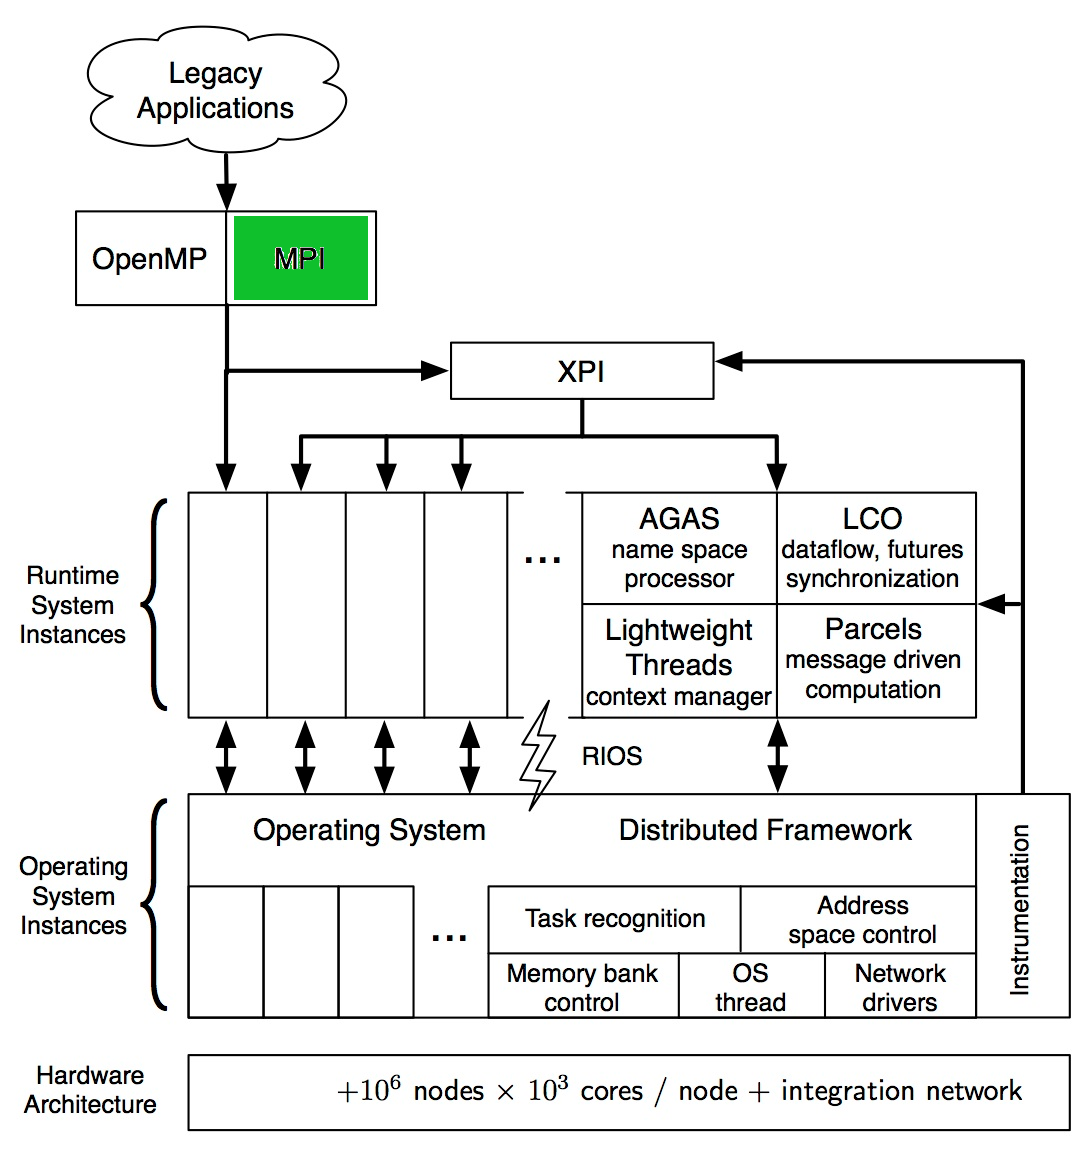
\includegraphics[scale=0.75]{images/openx.png}
\caption[The OpenX Software Architecture]{The OpenX Software Architecture~\cite{xpress}}
\label{fig:openx}
\end{figure}

\section{Design Principles}
\label{sec:design}
The main goal of this project that led to the development of HPX-RTE was to provide facilities for MPI applications to compile and run the exact same way in exascale software stack environment and be compatible with HPX runtime environment. This goal is achieved by replacing the current runtime environment (ORTE) with a new runtime environment developed from scratch to take advantage of the API provided by HPX. This choice was made by having a set of design principles in mind.

\begin{itemize}
\item \textbf{Modularity}\\
  Utilizing the modular structure of the Open MPI project, there is a framework dedicated to the runtime environment (rte) in OMPI layer. This framework is designed to provide the interfce necessary for different runtime environments (Figure \ref{fig:MCA-hpx-rte}). This allows different runtime environments to coexist independently inside the Open MPI project and be chosen by users based on their environment and application needs and priorities.

\begin{figure}[ht]
\centering
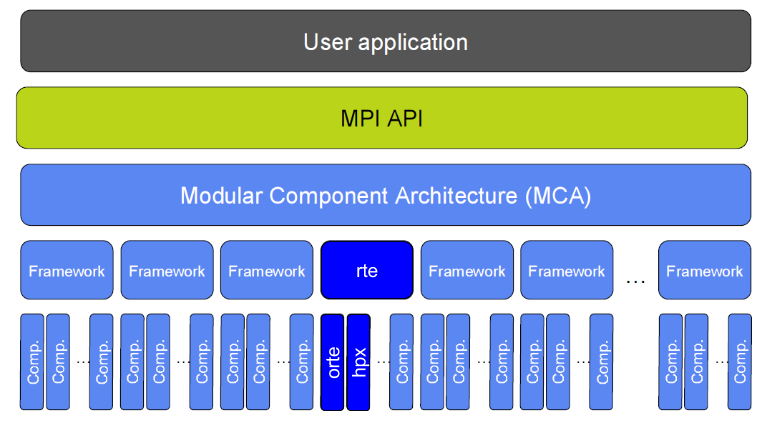
\includegraphics[scale=0.5]{images/MCA-hpx-rte.png}
\caption[Modular Component Architecure with rte Framework]{Modular Component Architecure with rte Framework}
\label{fig:MCA-hpx-rte}
\end{figure}
  
\item \textbf{Functionality}\\
  The main focus of this work is to have the MPI applications work on HPX infrastructure. To do this, most of the effort is put on having the functionality in place before tackling any possible consequences such as its effect on performance, efficiency, or power consumption. Although every possible consideration has been takeninto account not to introduce sources of performance degradation, such potential side effects could still happen. Those may be the topic for other studies after having the new runtime environment in place and functional.
  
\item \textbf{Simplicity}\\
  Simplicity is a key factor is the design of HPX-RTE. We have avoided introducing any unnecessary algorithm or functionality. Implementing the required API, we have tried to keep implementation as simple and straightforward as possible.

\item \textbf{Code Reuse}\\
  HPX-RTE relies on a number of advanced features and concepts provided by the HPX API. Therefore, there was no need to reimplement what was already done. We have tried to take those features to a new level by integrating them tightly into the implementation of HPX-RTE.

\end{itemize}

\section{Architecture}
\label{sec:architecture}

HPX-RTE is designed to replace the functionality of current Open MPI runtime (ORTE). Figure \ref{fig:open-mpi-layers-hpx-rte} illustates the logical layers of Open MPI software using \mbox{HPX-RTE} as its runtime environment. The modular component architecture of Open MPI facilitates the implementation of this design.

The required functinality for HPX-RTE is implemented as a component of the runtime environment (rte) framework (Figure \ref{fig:MCA-hpx-rte}) in OMPI layer. This design dictates a number of changes outside the rte framework. We will discuss those changes in the implementation section.

\begin{figure}[ht]
\centering
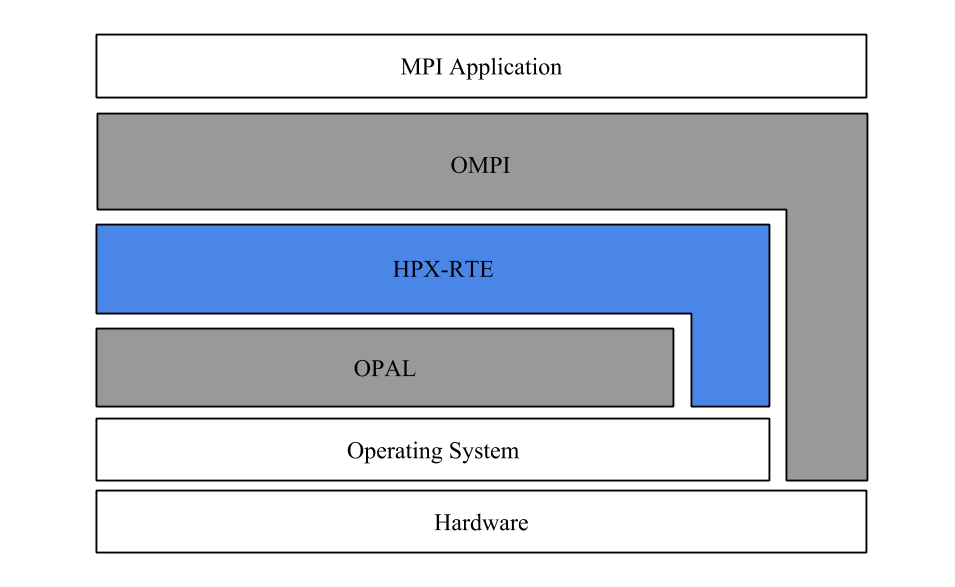
\includegraphics[scale=0.45]{images/open-mpi-layers-hpx-rte.png}
\caption[Open MPI Layers using HPX-RTE]{Open MPI Layers using HPX-RTE}
\label{fig:open-mpi-layers-hpx-rte}
\end{figure}

\section{Runtime Environement Requirements}
\label{sec:rte-requirements}
The rte framework inside OMPI layer of Open MPI defines a required set of data structures and functions that every runtime environment component needs to provide implementation for~\cite{gabriel04:_open_mpi}:

\subsection{Process Name Objects and Operations}

\begin{enumerate}
\item \verb|ompi_jobid_t| \textbf{and} \verb|ompi_vpid_t|\\
  These two need to be defined as integer types. The jobid must be unique for a given \verb|MPI_COMM_WORLD| capable of connecting to another \verb|OMPI_COMM_WORLD| and the vpid will be the process's rank in \verb|MPI_COMM_WORLD|.

\item \verb|ompi_process_name_t|\\
  This is a struct that must contain at least two fields of type integer:
  \begin{enumerate}
  \item \verb|ompi_jobid_t| jobid
  \item \verb|ompi_vpid_t| vpid
  \end{enumerate}

\item \verb|OMPI_NAME_PRINT|\\
  When given a pointer to \verb|ompi_process_name_t|, this macro has to print a process name. The output format has to be a single string representing the name. This function should be thread-safe for multiple threads to call simultaneously.
  
\item \verb|OMPI_PROC_MY_NAME|\\
  A pointer to a global variable containing the \verb|ompi_process_name_t| for this process.
  
\item \verb|OMPI_NAME_WILDCARD|\\
  A wildcard name.
  
\item \verb|ompi_rte_compare_name_fields|\\
  A function used to compare fields in the \verb|ompi_process_name_t| struct. The function prototype must be of the form:
  \begin{lstlisting}[language=C]
    int ompi_rte_compare_name_fields(
        ompi_rte_cmp_bitmask_t mask,
        ompi_process_name_t *name1,
        ompi_process_name_t *name2);
  \end{lstlisting}
                                         The bitmask must be defined to indicate the fields to be used
        in the comparison. Fields not included in the mask must be ignored.
        Supported bitmask values must include:
           b. \verb|OMPI_RTE_CMP_JOBID|
           c. \verb|OMPI_RTE_CMP_VPID|
           d. \verb|OMPI_RTE_CMP_ALL|
         \item \verb|uint64_t ompi_rte_hash_name|(name) - return a string hash uniquely representing the \verb|ompi_process_name| passed in.
       \item \verb|OMPI_NAME| - an Opal DSS constant for a handler already registered to serialize/deserialize an \verb|ompi_process_name_t| structure.

\end{enumerate}


\iffalse
         
 (b) Collective objects and operations
     1. \verb|ompi_rte_collective_t| - an OPAL object used during RTE collective operations such as modex and barrier. It must be an \verb|opal_list_item_t| and contain the following fields:
           a. id (ORTE type: \verb|int32_t|)
           b. bool active
              flag that user can poll on to know when collective
              has completed - set to false just prior to
              calling user callback function, if provided
     2. \verb|ompi_rte_modex| - a function that performs an exchange of endpoint information to wireup the MPI transports. The function prototype must be of the form:
        int \verb|ompi_rte_modex(ompi_rte_collective_t *coll)|;
        At the completion of the modex operation, the coll->active flag must be set to false, and the endpoint information must be stored in the modex database.
        This function must have barrier semantics across the \verb|MPI_COMM_WORLD| of the calling process.
     3. \verb|ompi_rte_barrier| - a function that performs a barrier operation within the RTE. The function prototype must be of the form:
        int \verb|ompi_rte_barrier(ompi_rte_collective_t *coll)|;
        At the completion of the barrier operation, the coll->active flag must be set to false

 (c) Process info struct
     1. \verb|ompi_process_info_t| - a struct containing info about the current process.
        The struct must contain at least the following fields:
           a. \verb|app_num| -
           b. pid - this process's pid.  Should be same as getpid().
           c. \verb|num_procs| - Number of processes in this job (ie, MCW)
           d. \verb|my_node_rank| - relative rank on local node to other peers this run-time instance knows about.  If doing dynamics, this may be something different than \verb|my_local_rank|, but will be \verb|my_local_rank| in a static job.
           d. \verb|my_local_rank| - relative rank on local node with other peers in this job (ie, MCW)
           e. \verb|num_local_peers| - Number of local peers (peers in MCW on your node)
           f. \verb|my_hnp_uri| -
           g. \verb|peer_modex| - a collective id for the modex operation
           h. \verb|peer_init_barrier| - a collective id for the barrier during \verb|MPI_Init|
           i. \verb|peer_fini_barrier| - a collective id for the barrier during \verb|MPI_Finalize|
           j. \verb|job_session_dir| -
           k. \verb|proc_session_dir| -
           l. nodename - a string representation for the name of the node this
              process is on
           m. cpuset -
     2. \verb|ompi_process_info| - a global instance of the \verb|ompi_process_t| structure.
     3. \verb|ompi_rte_proc_is_bound| - global boolean that will be true if the runtime bound the process to a particular core or set of cores and is false otherwise.

 (d) Error handling objects and operations
     1. void \verb|ompi_rte_abort(int err_code, char *fmt, ...)| - Abort the current process with the specified error code and message.
     2. int \verb|ompi_rte_abort_peers(ompi_process_name_t *procs, size_t nprocs)| -
        Abort the specified list of peers
     3. \verb|OMPI_ERROR_LOG(rc)| - print error message regarding the given return code
     4. \verb|ompi_rte_register_errhandler| - register a callback function for the RTE to report asynchronous errors to the caller

 (e) Init and finalize objects and operations
     1. \verb|ompi_rte_init| - a function to initialize the RTE. The function
        prototype must be of the form:
        int \verb|ompi_rte_init(int *argc, char ***argv)|;
     2. \verb|ompi_rte_finalize| - a function to finalize the RTE. The function
        prototype must be of the form:
        \verb|int ompi_rte_finalize(void)|;
     3. void \verb|ompi_rte_wait_for_debugger(void)| - Called during \verb|MPI_Init|, this function is used to wait for debuggers to do their pre-MPI attach.
        If there is no attached debugger, this function will not block.

 (f) Database operations
     1. \verb|ompi_rte_db_store| - a function to store modex and other data in
        a local database. The function is primarily used for storing modex
        data, but can be used for general purposes. The prototype must be
        of the form:
        int \verb|ompi_rte_db_store|(const \verb|ompi_process_name_t| *proc,
                              const char *key, const void *data,
                              \verb|opal_data_type_t| type);
        The implementation of this function must store a COPY of the data
        provided - the data is NOT guaranteed to be valid after return
        from the call.
     3. \verb|ompi_rte_db_fetch| -
        NOTE: Fetch accepts an '\verb|ompi_proc_t|'.
        int \verb|ompi_rte_db_fetch|(const struct \verb|ompi_proc_t| *proc,
                              const char *key,
                              void **data,
                              \verb|opal_data_type_t| type);
     4. \verb|ompi_rte_db_fetch_pointer| -
        NOTE: Fetch accepts an '\verb|ompi_proc_t|'.
        int \verb|ompi_rte_db_fetch_pointer|(const struct \verb|ompi_proc_t| *proc,
                                      const char *key,
                                      void **data,
                                      \verb|opal_data_type_t| type);
     5. Pre-defined db keys (with associated values after \verb|rte_init|)
        a. \verb|OMPI_DB_HOSTNAME|
        b. \verb|OMPI_DB_LOCALITY|

  (g) Communication support

\section{Challenges}
\label{sec:challenges}

%\subsection{C and C++}
%\subsection{Imperfect Abstraction in ORTE}
%\subsection{Fundamental Differences}
%\subsection{Configuration Logic}



\section{Implementation}
\label{sec:implementation}
MPI system level adjustment, and change of configuration logic

what we have done?
Open MPI has an abstraction layer for runtime environments.
We provide that abstraction layer using hpx.
The abstraction is imperfect(lack of documentation,
not perfect interface independences)
Key components we had to develop?
- distributed key-value store and fetch using hpx actions
- barrier (synchronization point) using hpx actions
- translation table from hpx localities to mpi ranks
- populating some internal data structures
- extract and populate some key-value pairs into the db:
some are set in orte layer and used in ompi layer
- hacking the configure logic to detect and handle boost and HPX libraries
and modify the generated make files accordingly
- using c++ to compile a number of components
- manually exclude some components that are deeply entangled with rte
- intercepting printf from c code to see the output


current status:
- hpx 0.9.9
- openmpi 1.8.4
- restrctions: - one rank per locality
- launch with ssh
- communication protocols:
tcp: - tests (including communication) are running now
shared memory: -not tried recently, it did not work early on

questions/topics to discuss:
- os functionalities and interactio with hpx: fork, pipe, mmap
- slurm integration

\fi

\section{HPX-RTE Requirements}
open mpi
hpx
boost

features:
automatic detection of boost installation and hpx installation
